% To compile: pdflatex file.tex
\documentclass[11pt]{article}
\usepackage{fullpage}
\usepackage{pgffor}
\usepackage{amssymb}
\usepackage{bm}
\usepackage{mathtools}
\usepackage{verbatim}
\usepackage{appendix}
\usepackage{graphicx}
\usepackage{color}
\usepackage{subfig}
\usepackage{url} % for underscore in footnote
\usepackage[UKenglish]{isodate} % for: \today
\cleanlookdateon                % for: \today
\usepackage{natbib} % Can remove if no bibliography. bibtex
%\pagestyle{empty} % Removes page number. Graphs too big.

\def\wl{\par \vspace{\baselineskip}\noindent}
\def\beginmyfig{\begin{figure}[h]\center}
\def\endmyfig{\end{figure}}
\def\ds{\displaystyle}
\def\tu{\textunderscore}
\definecolor{grey}{rgb}{.2,.2,.2}
\definecolor{lgrey}{rgb}{.8,.8,.8}
\def\hline{ \textcolor{lgrey}{\hrulefill} }
\newcommand{\m}[1]{\mathbf{\bm{#1}}} % Serif bold math
\def\ds{\displaystyle}                                                    
\def\inv{^{\raisebox{.2ex}{$\scriptscriptstyle-1$}}}
\def\pm{^{\raisebox{.2ex}{$\scriptscriptstyle\prime$}}}
\def\norm#1{\left\lVert#1\right\rVert}

% \def for THIS ASSIGNMENT!!!%%%%%%%%%%%%%%%%%%%

\begin{document}
% my title:
\begin{center}
  {\huge \textbf{Review of the Spatial Dirichlet Process}
    \footnote{\url{https://github.com/luiarthur/bnp_hw/project/bnp_spatialDP}}
  }\\
  \wl
  UCSC AMS 241 Course Project\\
  \noindent\today\\
  Arthur Lui\\
  \hline
\end{center}

\noindent
This project is a review of the spatial Dirichlet process (SDP) developed by
\cite{sdp}. I will first discuss how to model using the SDP, then examine
properties of the model through a data analysis.

\section{Spatial Dirichlet Process Modeling}
\noindent
To denote realizations from point-referenced spatial data, we use $\{y(s): s\in
S\}, S \subset R^d$, where $d$ is the dimension of $S$. We observe data only at
a subset of all possible points in $S$, $\m s^{(n)}=(s_1,...,s_n)$ . Typically,
this type of data is modeled by a Gaussian process (GP). However, the
assumption that the data arises from a GP is often a restriction.  we may
want to allow deviation from a Gaussian random field. An SDP prior can be put
on the random field and have a Gaussian process as the baseline distribution.
Required for the model are replicates at each point. That is we need the full
dataset to consist of a collection of vectors $\m y_t = (y(s_1),...,y(s_n))$,
$t=1,,,.T$. Note that the points $s_i$ can be a pair of latitudes and
longitudes.\\

\noindent
We can construct the model as follows:
\[
  \begin{array}{rclcl}
    %\m y_t &|& \m\theta_t,\beta,\tau^2 &\overset{ind.}{\sim}&\text{Normal}_n(\m\theta_t+ \m x_t\beta,
    \m y_t &|& \m\theta_t,\beta,\tau^2 &\overset{ind.}{\sim}&\text{N}_n(\m\theta_t+ \m{1_n}\beta,
    ~\tau^2\m I_n), ~~_{t=1,...,T}\\
    \m\theta_t &|& G^{(n)} &\overset{i.i.d.}{\sim}& G^{(n)}, ~~_{t=1,...,T} \\
    G^{(n)} &|& \alpha, \sigma^2, \phi &\sim&
      \text{DP}(~\alpha,G_0^{(n)}~\text{N}_n(\m 0_n,\sigma^2H_n(\phi)) ~) \\
    \\
            && \beta, \tau^2 &\sim& \text{N}(m,s^2) \times \text{IGamma}(a_{\tau^2}=2,b_{\tau^2}) \\
            && \alpha &\sim& \text{Gamma}(a_\alpha,b_\alpha) \\
            && \sigma^2 &\sim& \text{IGamma}(b_{\sigma^2}=2,b_{\sigma^2}) \\
            && \phi &\sim& \text{Uniform}(0,b_\phi) \\
  \end{array}
\]
where $H_n(\phi)$ is a covariance function, for example, the exponential
covariance function with decay parameter $\phi$. (i.e.  $(H_n(\phi))_{ij} =
\exp\left\{-\phi~\norm{s_i-s_j}\right\}$.)\\

\noindent
Here, $\m\theta_t$ are the location-specific mean deviations from a grand mean
$\beta$ across the $n$ spatial locations. Notice that clustering can result
among the $\m\theta_t$'s. This may be useful when our $\theta_t$'s are indexed
by time and we want to learn how the observations are clustered in time.  Also
notice that if we replaced the prior for the $\m\theta$ the baseline
distribution used, we get a Gaussian process.  And as $\alpha \rightarrow
\infty$, $\m\theta_t$ become i.i.d. $G_0^{(n)}$ conditional on the
hyperparameters. We assume $\m y_t$ to be independent and multivariate
normal with no correlation. That is, the covariance is $\tau^2 \m I_n$.
The $\m y_t$'s are simply modeled as a mixture of multivariate normals.\\

\subsection{Prior Specification}
The overall mean $\beta$ modeled with a normal prior. In modeling maximum
temperatures, it is appropriate to use a reasonably informative prior. In the
following data analysis, a prior mean of 30 and a prior variance of 5 were
used.  \cite{sdp} suggests for priors for $\sigma^2$ and $\tau^2$ Inverse-Gamma
priors with parameters $(2,b_{\sigma^2}$ and $(2,b_{\tau^2})$ respectively.
This corresponds to a prior mean of $b_{\sigma^2}$ and $b_{\tau^2}$ and
infinite variance for the two parameters. For the data analysis below, 
I used fixed variances as the model could not learn their values.
With a $T$ of only 20, it appears that posterior learning could not occur.
\cite{sdp} states that ``practical experience... suggests that there is
posterior learning for $[\alpha]$ when sampling sizes are moderate to large''.
Again $\phi$, which determines the rate of decay in the exponential decay function,
was fixed. The prior for $\alpha$ chosen such that the prior mean and variance were 1 and 
and 100 respectively.\\

\noindent
Note that all the above priors except that for $\phi$ are conjugate. And yields
the following complete conditionals that can be used in a Gibbs sampler.
\[\def\arraystretch{1.4}
  \begin{array}{rclcl}
    \beta &|& \m y, \m\theta, \tau^2  &\sim& \text{N}(
      \frac{\tau^2m + s^2\sum_{t=1}^T\sum_{i=1}^n(y_{it}-\theta_{it})}{\tau^2+Tns^2},
      \frac{s^2\tau^2}{\tau^2+Tns^2}) \\
    \tau^2 &|& \m y, \m\theta, \beta  &\sim& \text{IG}(a_{\tau^2}+\frac{nT}{2},
    b_{\tau^2}+\frac{\sum_{t=1}^T (\m\mu_t-\beta \m1_n)'(\m\mu_t-\beta \m1_n)}{2})\\
    %p(\sigma^2 &|& \m\theta_t^*, T^*, \m y, \sigma^2) &\propto& [\sigma^2]\prod_{t=1}^{T^*}
    %  ~\text{N}_n(\m\theta_t^* | \m 0_n,\sigma^2H_n(\phi)) ~)\\
    \sigma^2 &|& \m\theta^*, T^*, \m y, \sigma^2 &\sim& \text{IG}(a_{\sigma^2}+\frac{nT^*}{2},
      %b+\frac{\sum_{t=1}^{T^*}\m\theta^*'Hn^{-1}(\phi)\m\theta^*}{2})\\
    b_{\sigma^2}+\frac{\sum_{t=1}^{T^*}\m\theta_t^{*'} H_n^{-1}(\phi)\m\theta_t^*}{2})\\
    %p(\phi &|& \m\theta_t^*, T^*, \m y, \sigma^2) &\propto& \prod_{t=1}^{T^*} 
    %  ~\text{N}_n(\m\theta_t^* |\m 0_n,\sigma^2H_n(\phi)) ~)\\
    p(\phi &|& \m\theta^*, T^*, \m y, \sigma^2) &\propto& 
    [\phi]|H_n(\phi)|^{-T^*/2} \exp\left(-\frac{\sum_{t=1}^{T^*}\m\theta_t^{*'} H_n^{-1}(\phi)\m\theta_t^*}{2\sigma^2}\right)\\
    \eta &|& \alpha, \m y &\sim& \text{Beta}(\alpha+1,T)\\
    p(\alpha &|& T^*, \m y) &=& (\epsilon)~\gamma(\alpha | a_\alpha+T^*, b_\alpha-\log(\eta)) +\\
             &&&&(1-\epsilon)~\gamma(\alpha | a_\alpha+T^*-1, b_\alpha-\log(\eta))\\
  \end{array}
\]
where $\m\mu_t=\m{y_t -\theta_t} $, $\eta$ is an auxiliary variable introduced
to make the prior for $\alpha$ conjugate, $\gamma$ is the gamma density
function with the mean and rate parameterization, and 
$\epsilon = \ds\frac{a_\alpha +T^* - 1}{ n(b_\alpha-\log(\eta)) + a_\alpha +T^* -1}$.\\

\noindent
As $\m\theta_t$ has prior conjugacy, we can use the algorithm provided by \cite{escobar}
\def\mm{\m{y_t}-\m{1_n}\beta}
\[\def\arraystretch{1.4}
  \begin{array}{rllcl}
    \m\theta_t &|& y_t,\beta,\tau^2,\sigma^2,\phi &\sim& \text{N}_n(\tau^{-2}\m\Lambda(\mm), \m\Lambda)\\
               && q0 &=& |\Lambda|^{1/2} \\
               %&&&& \times \exp\left\{.5\tau^{-2}(\mm)'(\m{I_n}-\tau^{-2}\m\Lambda)(\mm)\right\}\\
               &&&& \times \exp\left\{\frac{(\mm)'(\m{I_n}-\tau^{-2}\m\Lambda)(\mm)}{2\tau^2}\right\}\\
               &&&& \times [(2\pi\tau^2\sigma^2)^{n/2} |H_n(\phi)|^{1/2}]^{-1}\\
  \end{array}
\]
where $\m\Lambda = [\tau^{-2}\m I_n + \sigma^{-2} H_n^{-1}(\phi)]^{-1}$.

\subsection{Prediction at Unobserved Locations}
Often, spatial modeling is used for prediction at unobserved locations
(kriging). If we were able to observe the replicates at new locations, we
get the following full Bayesian model
\[
  \prod_{t=1}^{T} [\m y_t|\m\theta_t,\beta,\tau^2]
  \prod_{t=1}^{T} [\tilde{\m y_t}|\tilde{\m\theta_t},\beta,\tau^2]
  \prod_{t=1}^{T} [(\m\theta_t,\tilde{\m\theta_t})|G^{(n+m)}][G^{(n+m)}|\alpha,\sigma^2,\phi]
  [\tau^2][\alpha][\sigma^2][\phi]
\]
where $\tilde{\m y_t}$ and $\tilde{\m\theta_t}$ are the \textbf{unobserved}
replicate and it's location specific mean at new locations
$(y_t(\tilde{s_1}),...,y_t(\tilde{s_m}))$, for $t=1,...,T$. The second term can
be integrated from the multivariate normal likelihood (this is done by simply
taking the corresponding terms in our likelihood away from the model). Also, 
after marginalizing over $G^{(n+m)}$ we obtain the following expression
\[
  \left(\prod_{t=1}^{T} [\m y_t|\m\theta_t,\beta,\tau^2]\right)
  [(\theta_1,\tilde{\theta_1}),...,(\theta_T,\tilde{\theta_T})|\alpha,\sigma^2,\phi]
  [\tau^2][\alpha][\sigma^2][\phi].
\]
This expression can be further rewritten as 
\[
  \left(\prod_{t=1}^{T} [\m y_t|\m\theta_t,\beta,\tau^2]\right)
  [(\theta^*,\tilde{\theta^*})|T^*,\sigma^2,\phi][\m w, T^*|\alpha,\sigma^2,\phi]
  [\tau^2][\alpha][\sigma^2][\phi],
\]
where the $(\theta^*,\tilde{\theta^*})$ are the unique $\m\theta_t$ which arise
i.i.d. from $G_0^{(n+m)}$. That is
$[(\theta^*,\tilde{\theta^*})|T^*,\sigma^2,\phi]
=\prod_{j=1}^{T^*}\text{N}_{n+m}(\theta^*_j,\tilde{\theta^*_j}~|~\m
0_{n+m},\sigma^2 H_{n+m}(\phi))$. Finally, the model can be expressed as
\[
  \left(\prod_{t=1}^{T} [\m y_t|\m\theta_t,\beta,\tau^2]\right)
  \left(\prod_{t=1}^{T^*}[\tilde{\theta_j^*}| \theta_j^*,\sigma^2,\phi]\right)
  \left(\prod_{t=1}^{T^*}\text{N}_{n}(\theta^*_j~|~\m 0_{n},\sigma^2 H_n(\phi))\right)
  [\m w, T^*|\alpha,\sigma^2,\phi] [\tau^2][\alpha][\sigma^2][\phi],
\] or equivalently
\[
  \left(\prod_{t=1}^{T^*}[\tilde{\theta_j^*}| \theta_j^*,\sigma^2,\phi]\right)
  \left(\prod_{t=1}^{T} [\m y_t|\m\theta_t,\beta,\tau^2]\right)
  \left(\prod_{t=1}^{T^*}\text{N}_{n}(\theta^*_j~|~\m 0_{n},\sigma^2 H_n(\phi))\right)
  [\m w, T^*|\alpha,\sigma^2,\phi] [\tau^2][\alpha][\sigma^2][\phi].
\]
Based on the expression above, the joint posterior
$[(\m\theta^*,\tilde{\m\theta^*}),\m w, T^*,\beta,\tau^2,\alpha,\sigma^2,\phi|\text{data}]$
can be decomposed into 
\[
  \left(\prod_{t=1}^{T^*}[\tilde{\theta_j^*}| \theta_j^*,\sigma^2,\phi]\right)
  [~\m\theta^*,\m w, T^*,\beta,\tau^2,\alpha,\sigma^2,\phi|\text{data}~].
\]
The second term can be is the joint posterior in the SDP model. So, we can employ 
the following algorithm to the MCMC outputs to obtain posterior draws for 
$\prod_{t=1}^{T^*}[\tilde{\theta_j^*}| \theta_j^*,\sigma^2,\phi]$: 
for each $b = 1,...,B$, sample from $[\tilde{\theta_j^*}| \theta_j^*,\sigma^2,\phi]$
for each $j = 1,...,T^*$. Notice that 
\[
  \tilde{\theta_j^*}|\theta_j^*,\sigma^2,\phi \sim \text{N}_m(\m 0_m+\m S_{12}\m S_{22}^{-1}(\theta_j-\m 0_n),
  ~~\m S_{11} - \m S_{12} \m S_{22}^{-1} \m S_{21})
\]
where $\m S = \sigma^2 H_{n+m}(\phi)$, and the subsequent submatrices are defined as follows:
$\m S_{11} = \sigma^2 H_{1:m,~1:m}(\phi)$,
$\m S_{12} = \sigma^2 H_{1:m,~m+1:m+n}(\phi)$,
$\m S_{22} = \sigma^2 H_{m+1:m+n,~m+1:m+n}(\phi)$,
$\m S_{21} = \sigma^2 H_{m+1:m+n,~1:m}(\phi)$.\\
To obtain posterior predictives at the new locations, we further draw values for 
$(\tilde{\m y_{0b}},\m y_{0b})$ from $\text{N}_{m+n}(\beta_b\m 1_{m+n}+(\tilde\theta_{0b},\theta_{0b}),\tau^2\m I_{m+n})$.

\section{Data Analysis}
The data used for this study was gathered from The Atmospheric Science Data
Center at NASA. The script used to parse this dataset can be found at the
referenced website
\footnote{\url{https://github.com/luiarthur/bnp_hw/tree/master/project/bnp_spatialDP/data/retrieve}}.
The data consists of daily averaged maximum temperatures at 10 meters for every
July from 1985 to 2004, at 100 locations. (There was available every month
average within the years and for more locations, but to save on computation,
only a subset of the data was retrieved and used.) Figure \ref{fig:dat} shows
the average maximum daily temperatures at 100 locations in July 1989, with
hotter regions in dark red and cooler regions in dark blue. It can be seen and expected that
in the northern regions and along the coast, temperatures are lower; and in the
southern and inland regions, temperatures are higher. We fit the mentioned model
to our data using the suggested prior specification (with the exception of 
fixing the variances).\\
\beginmyfig 
  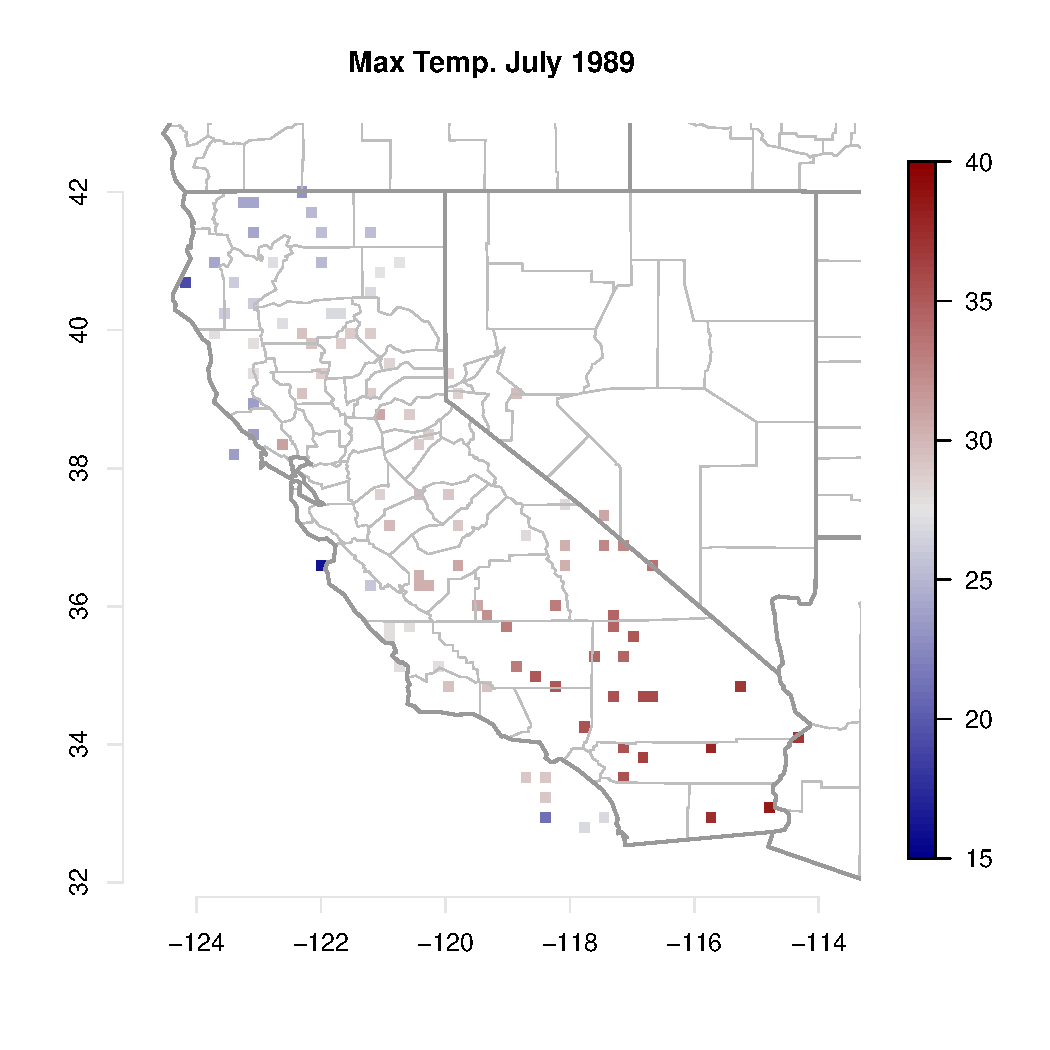
\includegraphics[scale=.6]{../graphs/july1989.pdf} 
  \caption{Average maximum daily temperatures at various locations in the state of California in 1989. 
  Warmer areas are dark red and cooler locations are dark blue.}
  \label{fig:dat}
\endmyfig

\noindent
We plot the mean of the data (mean temperatures at each location) side by side
with the posterior predictive mean in Figure \ref{fig:postmean}. We see that
the model smoothly interpolates the temperatures between locations of known
temperature. The model borrows information from closer locations and less
information from grid points far away. Far from the locations with data, the
temperatures return the the mean $\beta$.

\beginmyfig
  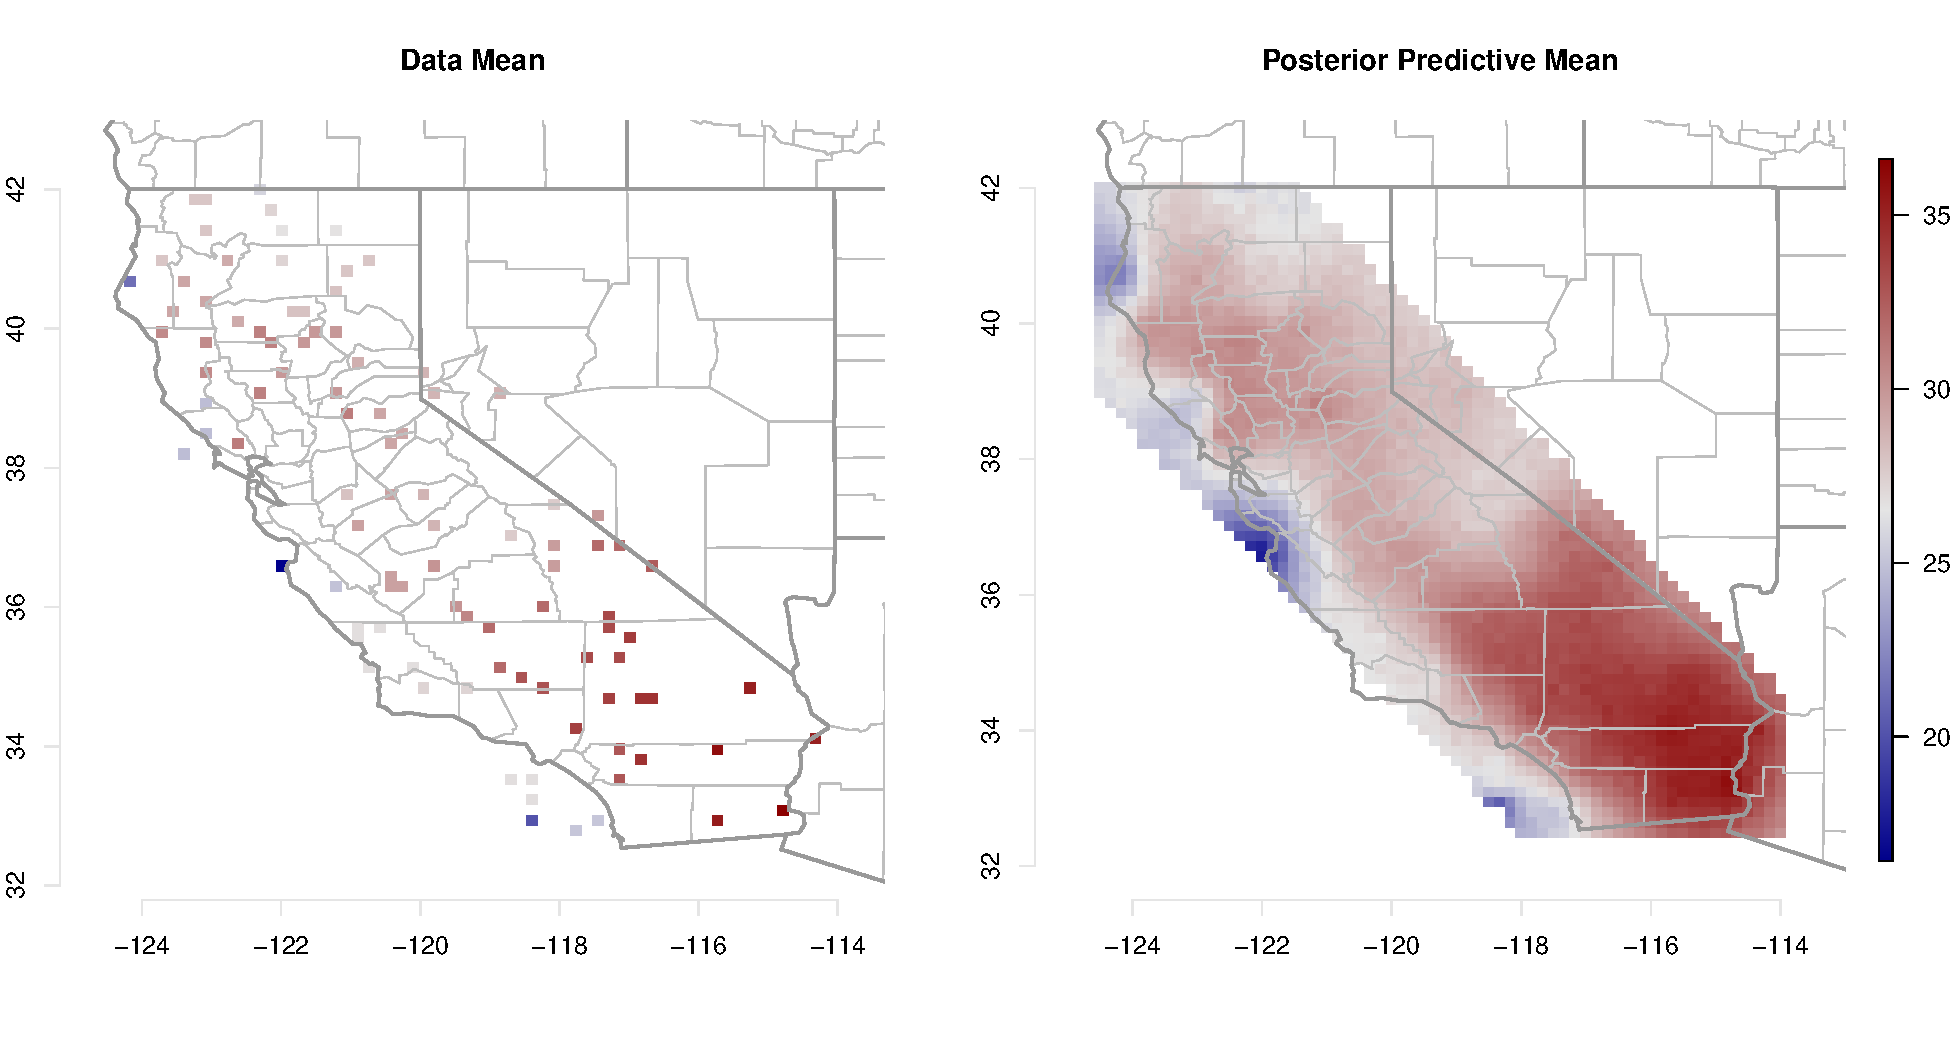
\includegraphics[scale=.5]{../graphs/postpredmean.pdf}
  \caption{Left: Average of the average maximum daily temperatures at recorded locations
  in California.
  Right: Predicted average maximum daily temperatures at various locations in
  the state of California for a new year.  Warmer areas are dark red and cooler
  locations are dark blue.}
  \label{fig:postmean}
\endmyfig

\noindent
The posterior predictive variance in Figure \ref{fig:postvar}.  The variance in
the posterior predictive is large (about 20 everywhere). I suspect this is due
to the small amount of data ($T=20$). With more data, which is available this
can be remedied. It should be noted that in $C++$ fitting the model with 2500
MCMC iterations took 3 minutes.  Fitting the model with more data can be easily
accommodated and quick. In predicting at new locations, matrix inversions can
take a long time with large matrices, but this can be sped up by
parallelization on larger systems.

\beginmyfig
  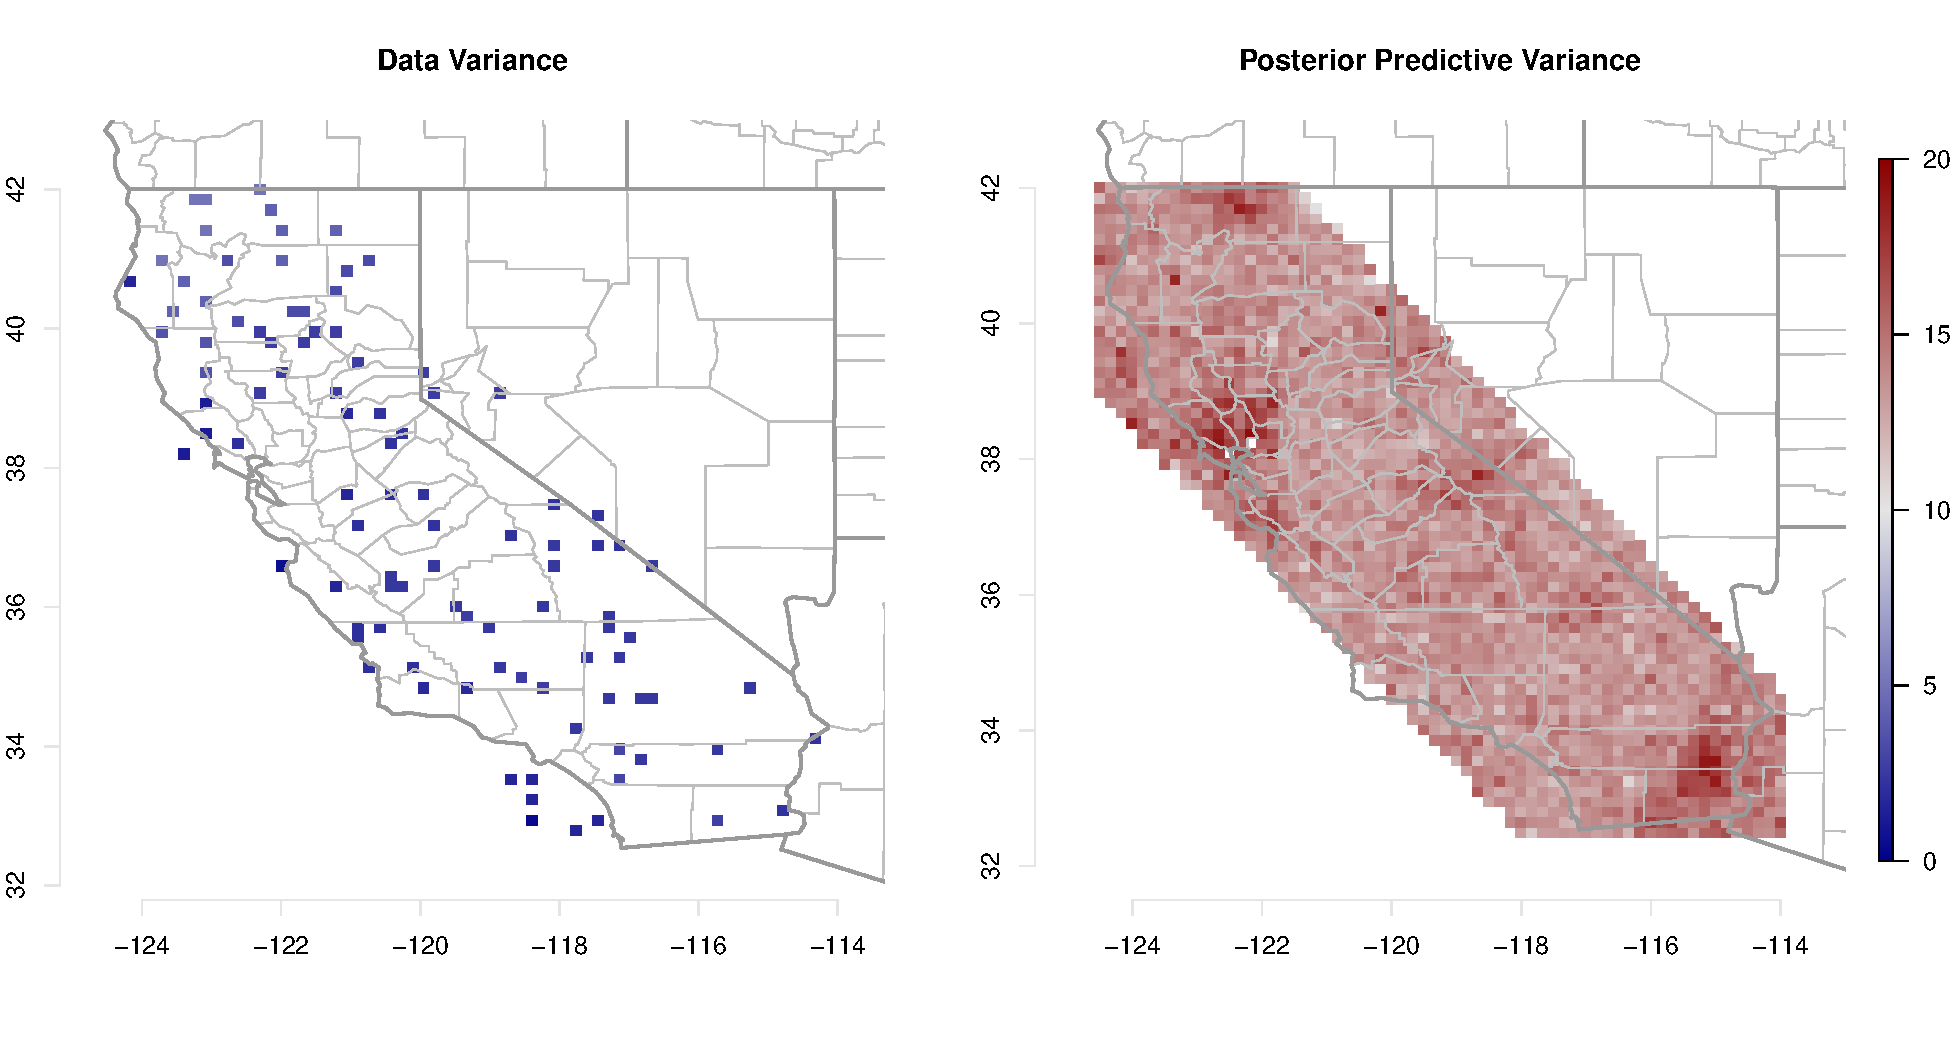
\includegraphics[scale=.5]{../graphs/postpredvar.pdf}
  \caption{Left: Variance of the average maximum daily temperatures at recorded locations
  in California.
  Right: Predicted variance of the average maximum daily temperatures at various locations in
  the state of California for a new year.  Areas with higher variance are dark red and areas 
  with lower variance would be in dark blue. Almost all locations have high variance.}
  \label{fig:postvar}
\endmyfig

\section{Conclusions}
The spatial Dirichlet process provides a flexible framework for modeling
spatial data when stationarity and Gaussianity is not desireable. Clustering
can be induced (though not discussed here). Posterior predictive for new
locations can be done easily \textit{after} fitting the model with only the
locations in the data. So, predictions at new locations can be done in parallel
after fitting the model. It is worth noting that further information can be
harvested from the data by modeling the temporal structure. This topic 
has been explored using the SDP by \cite{tsdp}.

%%% Bibliography
\bibliographystyle{asabyu} % bibtex
\bibliography{sdp}         % bibtex
\end{document}
